\documentclass{article}[11pt]

\usepackage{amsmath}
\usepackage{amssymb}
\usepackage{nicefrac}

\usepackage{pdflscape}

\usepackage{upgreek}

\usepackage{bashful}

% No intendation
\setlength\parindent{0pt}

\usepackage{hyperref}

\usepackage{siunitx}
\sisetup{
  per-mode=fraction,
  fraction-function=\tfrac
}

\usepackage{listings}
  \lstset{
    basicstyle=\ttfamily,
    escapeinside=||,
    xleftmargin=1cm
  }

\usepackage{float}

\usepackage{longtable}

\usepackage{multirow}

\usepackage{tikz}
  \usetikzlibrary{patterns}
  \usetikzlibrary{arrows.meta}
  \usetikzlibrary{shapes.misc}
  \usetikzlibrary{calc}

\usepackage{pgfplots}

\usepackage{cleveref}
\crefmultiformat{equation}{(#2#1#3)}{ and~(#2#1#3)}{, (#2#1#3)}{ and~(#2#1#3)}


\usepackage{acronym}
\usepackage[acronym,nonumberlist]{glossaries}
\glsdisablehyper
\makeglossaries
\newacronym{spice}{SPICE}{Simulation Program with Integrated Circuit Emphasis}
\newacronym{lef}{LEF}{Library Exchange Format}
\newacronym{dft}{DFT}{Discrete Fourier Transform}
\newacronym{dtft}{DTFT}{Discrete-Time Fourier Transform}
\newacronym{fft}{FFT}{Fast Fourier Transform}
\newacronym{mosfet}{MOSFET}{Metal–Oxide–Semiconductor Field-Effect Transistor}
\newacronym{clm}{CLM}{Channel Length Modulation}
\newacronym{de}{DE}{differential equation}
\newacronym{soi}{SOI}{silicon-on-insulator}
\newacronym{ldo}{LDO}{low-dropout regulator}
\newacronym{ota}{OTA}{operational-transconductance amplifier}
\newacronym{ofa}{OFA}{operational-floating amplifier}

% literature
\usepackage[ backend=biber
           , isbn=true
           , sorting=none
           , style=ieee
           ]{biblatex}
\addbibresource{./../../literature.bib}

% definitions
\def \whatis       {Notes}
\def \title        {Fuubar}

\def \author       {Matthias Schweikardt}

\def \authorMail   {mschweikardt@posteo.de}

\def \authorGithub {mschweikardt}

\def \license      {CC BY-SA 4.0}
\def \licenseUrl   {https://creativecommons.org/licenses/by-sa/4.0/}

\def \date         {nodate}

\def \pdfurl       {https://mschweikardt.github.io/ee-notes/%
\bash[stdout]
IFS=/ 
var=($PWD)
echo ${var[-1]}
\END%
.pdf
}
\def \srcurl       {srcurl}


% Customize footer and header of document
\usepackage{fancyhdr}

% Access last page number
\usepackage{lastpage}

% Access last page number
\usepackage[thinc]{esdiff}

% Physics
\usepackage{physics}

% Comment environment
\usepackage{comment}

% Subcaptions
\usepackage{subcaption}

% Thicker lines in tables
\usepackage{booktabs}

% Indentation in footnote
\makeatletter
\renewcommand\@makefntext[1]{\leftskip=2em\hskip-0.5em\@makefnmark#1}
\makeatother         

% qty with the siunitx definition
\AtBeginDocument{\RenewCommandCopy\qty\SI}

% TikZ compatibility
\pgfplotsset{compat=1.18}


\makeatletter
\pgfmathdeclarefunction{myatan2}{2}{%
\begingroup%
  \pgfmathfloattofixed{#1}\edef\tempa{\pgfmathresult}%
  \pgfmathfloattofixed{#2}%
  \pgfkeys{pgf/fpu=false}%
  \pgfmathparse{atan2(\tempa,\pgfmathresult)}\pgfkeys{/pgf/fpu}%
  \pgfmathfloatparsenumber{\pgfmathresult}%
  \pgfmath@smuggleone\pgfmathresult%
\endgroup
}
\makeatother

\usepackage{tabularx}
\usepackage{amsmath}
\usepackage{amssymb}
\usepackage{nicefrac}

\usepackage{pdflscape}

\usepackage{upgreek}

\usepackage{bashful}

% No intendation
\setlength\parindent{0pt}

\usepackage{hyperref}

\usepackage{siunitx}
\sisetup{
  per-mode=fraction,
  fraction-function=\tfrac
}

\usepackage{listings}
  \lstset{
    basicstyle=\ttfamily,
    escapeinside=||,
    xleftmargin=1cm
  }

\usepackage{float}

\usepackage{longtable}

\usepackage{multirow}

\usepackage{tikz}
  \usetikzlibrary{patterns}
  \usetikzlibrary{arrows.meta}
  \usetikzlibrary{shapes.misc}
  \usetikzlibrary{calc}

\usepackage{pgfplots}

\usepackage{cleveref}
\crefmultiformat{equation}{(#2#1#3)}{ and~(#2#1#3)}{, (#2#1#3)}{ and~(#2#1#3)}


\usepackage{acronym}
\usepackage[acronym,nonumberlist]{glossaries}
\glsdisablehyper
\makeglossaries
\newacronym{spice}{SPICE}{Simulation Program with Integrated Circuit Emphasis}
\newacronym{lef}{LEF}{Library Exchange Format}
\newacronym{dft}{DFT}{Discrete Fourier Transform}
\newacronym{dtft}{DTFT}{Discrete-Time Fourier Transform}
\newacronym{fft}{FFT}{Fast Fourier Transform}
\newacronym{mosfet}{MOSFET}{Metal–Oxide–Semiconductor Field-Effect Transistor}
\newacronym{clm}{CLM}{Channel Length Modulation}
\newacronym{de}{DE}{differential equation}
\newacronym{soi}{SOI}{silicon-on-insulator}
\newacronym{ldo}{LDO}{low-dropout regulator}
\newacronym{ota}{OTA}{operational-transconductance amplifier}
\newacronym{ofa}{OFA}{operational-floating amplifier}

% literature
\usepackage[ backend=biber
           , isbn=true
           , sorting=none
           , style=ieee
           ]{biblatex}
\addbibresource{./../../literature.bib}

% definitions
\def \whatis       {Notes}
\def \title        {Fuubar}

\def \author       {Matthias Schweikardt}

\def \authorMail   {mschweikardt@posteo.de}

\def \authorGithub {mschweikardt}

\def \license      {CC BY-SA 4.0}
\def \licenseUrl   {https://creativecommons.org/licenses/by-sa/4.0/}

\def \date         {nodate}

\def \pdfurl       {https://mschweikardt.github.io/ee-notes/%
\bash[stdout]
IFS=/ 
var=($PWD)
echo ${var[-1]}
\END%
.pdf
}
\def \srcurl       {srcurl}


% Customize footer and header of document
\usepackage{fancyhdr}

% Access last page number
\usepackage{lastpage}

% Access last page number
\usepackage[thinc]{esdiff}

% Physics
\usepackage{physics}

% Comment environment
\usepackage{comment}

% Subcaptions
\usepackage{subcaption}

% Thicker lines in tables
\usepackage{booktabs}

% Indentation in footnote
\makeatletter
\renewcommand\@makefntext[1]{\leftskip=2em\hskip-0.5em\@makefnmark#1}
\makeatother         

% qty with the siunitx definition
\AtBeginDocument{\RenewCommandCopy\qty\SI}

% TikZ compatibility
\pgfplotsset{compat=1.18}


\makeatletter
\pgfmathdeclarefunction{myatan2}{2}{%
\begingroup%
  \pgfmathfloattofixed{#1}\edef\tempa{\pgfmathresult}%
  \pgfmathfloattofixed{#2}%
  \pgfkeys{pgf/fpu=false}%
  \pgfmathparse{atan2(\tempa,\pgfmathresult)}\pgfkeys{/pgf/fpu}%
  \pgfmathfloatparsenumber{\pgfmathresult}%
  \pgfmath@smuggleone\pgfmathresult%
\endgroup
}
\makeatother

\usepackage{tabularx}


\def \title  {Spectrum Properties}
\def \date   {June 12, 2025}

\def \pdfurl {https://mschweikardt.github.io/ee-notes/spectrum-properties.pdf}
\def \srcurl {https://github.com/mschweikardt/ee-notes/tree/main/notes/spectrum-properties}

\usepackage[scale=5]{draftwatermark}

\usepackage{tikz,pgfplots,filecontents,amsmath}

\newcommand{\ps}{\textcolor{cyan}{P_{\mathrm{S}}}}
\newcommand{\pone}{\textcolor{cyan}{P_{\mathrm{1}}}}
\newcommand{\pd}{\textcolor{purple}{P_{\mathrm{D}}}}
\newcommand{\ptwothree}{\textcolor{purple}{\textcolor{purple}{P_2}} + \textcolor{purple}{P_3} + \textcolor{purple}{...}}
\newcommand{\pdc}{\textcolor{olive}{P_{\mathrm{DC}}}}
\newcommand{\pzero}{\textcolor{olive}{P_{\mathrm{0}}}}
\newcommand{\pn}{\textcolor{orange}{P_{\mathrm{N}}}}

\begin{document}

\notetitle

\section{Introduction}
There are four different \textit{Fourier~transforms} to convert a time-domain 
signal in a frequency-domain representation (spectrum):
\begin{itemize}
  \item Fourier~Transformation
  \item Fourier~Series
  \item \gls{dtft}
  \item \gls{dft}
\end{itemize}
The spectrum of a signal, e.g. a voltage $v(t)$ or 
current $i(t)$, can be investigated with these transformations.
Various properties can be extracted from this spectrum to assess the quality
of the signal.

\medskip

Only the \gls{dft} is discrete both in the time and frequency domain.
For practical reasons, all kind of spectrum analysis should be processed on 
a computer, this is why only the \gls{dft} is applicable.

\begin{table}[H]
\centering
\caption{Variables}
\begin{tabular}{cl}
\toprule
\textbf{Variable}     & \textbf{Description}                     \\ \midrule
$x(t)$                & Time continous signal                    \\ 
$x[n]$                & Sampled version of  $x(t)$               \\ 
$x[n]$                & Sampled version of  $x(t)$               \\ 
$x_n$                 & Sampled version of  $x(t)$               \\ 
$y(t)$                & Output Signal (time domain)              \\ 
$t_{\mathrm{s}}$      & Settling time                            \\ \toprule
\end{tabular}
\label{tab:variables}
\end{table}

\section{Discrete Fourier Transform}


\begin{equation}\label{eq:ts}
T_{\mathrm{S}} = \frac{1}{f_{\mathrm{S}}}
\end{equation}

\begin{equation}\label{eq:xn}
x_n = x(n \cdot T_{\mathrm{S}})
\end{equation}



\begin{equation}\label{eq:xn}
\underline{X}[k] = \frac{1}{N} \sum_{n=0}^{N-1} 
  x[n] \cdot \exp\left(-j\frac{2\pi n}{N} k\right)
\end{equation}



\begin{equation}\label{eq:resolution}
\Delta f = \frac{f_{\mathrm{S}}}{N}
\end{equation}





$X(f)$

\section{Fast Fourier Transform}

\begin{itemize}
  \item The \gls{fft} is a algorithm for calculating the \gls{fft}.
  \item Best: $N$ is power of two, i.e. 2, 4, 16, 32,..
\end{itemize}

\begin{equation}\label{eq:xn}
\begin{aligned}
\underline{X}[k] 
&= \frac{1}{N} \sum_{n=0}^{N-1} x[n] \cdot \exp\left(-j\frac{2\pi n}{N} k\right) \\
&= \frac{1}{N} \sum_{n=0,2,...}^{N-2} x[n] \cdot \exp\left(-j\frac{2\pi n}{N} k\right) + \frac{1}{N} \sum_{n=1,3,...}^{N-1} x[n] \cdot \exp\left(-j\frac{2\pi n}{N} k\right)  \\
&= \frac{1}{N} \sum_{n=0}^{\frac{N}{2}-1} x[2n] \cdot \exp\left(-j\frac{2\pi 2n}{N} k\right) + \frac{1}{N} \sum_{n=0}^{\frac{N}{2}-1} x[2n+1] \cdot \exp\left(-j\frac{2\pi \left(2n+1\right)}{N} k\right)  \\
&= \frac{1}{N} \sum_{n=0}^{\frac{N}{2}-1} x[2n] \cdot \exp\left(-j\frac{2\pi 2n}{N} k\right) + \exp\left(-j\frac{2\pi}{N} k\right) \frac{1}{N} \sum_{n=0}^{\frac{N}{2}-1} x[2n+1] \cdot \exp\left(-j\frac{2\pi 2n}{N} k\right)  \\
&= \frac{1}{N} \sum_{n=0}^{\frac{N}{2}-1} x[2n] \cdot \exp\left(-j\frac{2\pi n}{\nicefrac{N}{2}} k\right) + \exp\left(-j\frac{2\pi}{N} k\right) \frac{1}{N} \sum_{n=0}^{\frac{N}{2}-1} x[2n+1] \cdot \exp\left(-j\frac{2\pi 2}{\nicefrac{N}{2}} k\right)  \\
\end{aligned}
\end{equation}

%y = 0.6 - 9.302778*x + 57.53056*x^2 - 103.4722*x^3 + 54.44444*x^4

\section{Coherent Sampling}


\section{Parasitic Effects}


\subsection{Aliasing}

The \textit{Nyquist–Shannon sampling theorem} says that a signal with maximal
frequency $f_{\mathrm{max}}$ must be sampled at least with the sampling 
frequency
\begin{equation}\label{eq:sampling-theorem}
f_{\mathrm{S}} = 2 \cdot f_{\mathrm{max}},
\end{equation}
i.e., twice the maximal frequency, such that the it can be 
reconstructed correctly.
When this principle is violated, aliasing occurs.




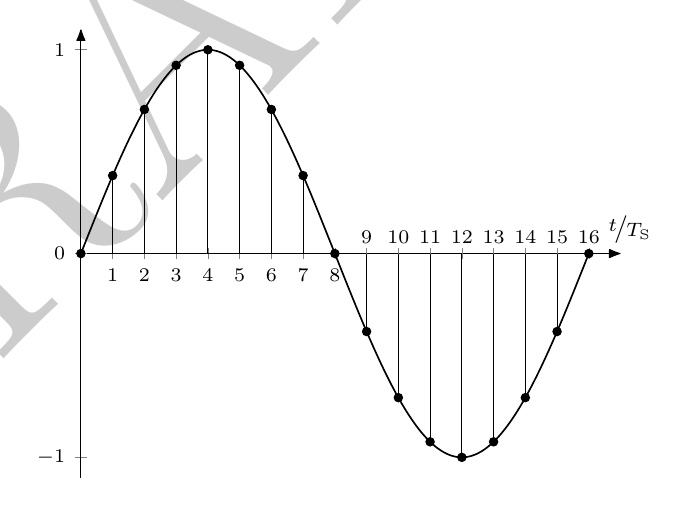
\begin{tikzpicture}
\begin{axis}[ axis x line=middle
            , axis y line=middle
            , xlabel={$\nicefrac{t}{T_{\mathrm{S}}}$}
            , ytick={-1,1}
            , extra y ticks={0}
            , extra y tick labels={0}
            , ymin=-1.1
            , ymax=1.1
            , yticklabel style = {font=\scriptsize}
            , axis line style={-{Latex[round]}}
            , xlabel style={at={(ticklabel* cs:0.96)},anchor=south west}
            , xmin=0
            , xmax=17
            , xtick={0, 1,...,8}
            , xticklabel style = {font=\scriptsize}
            , extra x ticks={9,10,...,16}
            , extra x tick labels={9,10,...,16}
            , extra x tick style={tick label style={above, yshift=0.5ex,font=\scriptsize}}
            ]
\addplot[semithick] plot[smooth,domain=0:16, samples=101] ({\x},{sin(360/16*\x)});
\addplot[ycomb, mark=*,mark size=1.5pt] plot[domain=0:16, samples=17] ({\x},{sin(360/16*\x)});
\end{axis}
\end{tikzpicture}


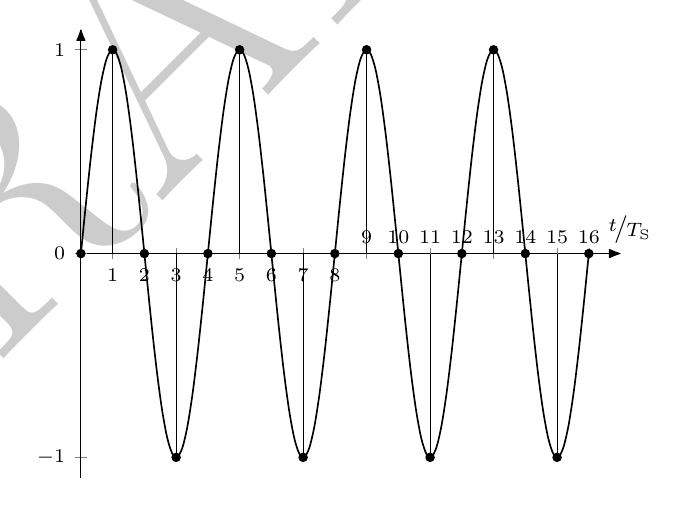
\begin{tikzpicture}
\begin{axis}[ axis x line=middle
            , axis y line=middle
            , xlabel={$\nicefrac{t}{T_{\mathrm{S}}}$}
            , ytick={-1,1}
            , extra y ticks={0}
            , extra y tick labels={0}
            , ymin=-1.1
            , ymax=1.1
            , yticklabel style = {font=\scriptsize}
            , axis line style={-{Latex[round]}}
            , xlabel style={at={(ticklabel* cs:0.96)},anchor=south west}
            , xmin=0
            , xmax=17
            , xtick={0, 1,...,8}
            , xticklabel style = {font=\scriptsize}
            , extra x ticks={9,10,...,16}
            , extra x tick labels={9,10,...,16}
            , extra x tick style={tick label style={above, yshift=0.5ex,font=\scriptsize}}
            ]
\addplot[semithick] plot[smooth,domain=0:16, samples=101] ({\x},{sin(360/16*4*\x)});
\addplot[ycomb, mark=*,mark size=1.5pt] plot[domain=0:16, samples=17] ({\x},{sin(360/16*4*\x)});
\end{axis}
\end{tikzpicture}

\begin{figure}[H]
  \centering
  \begin{tikzpicture}  
    \input{./../../tikzlib/figs/fft-aliasing-a.tex}   
  \end{tikzpicture}
  \caption{Aliasing}
  \label{fig:aliasing}
\end{figure}

\subsection{Spectral leakage}

\subsection{Interpolation}


\begin{tikzpicture}
\begin{axis}[ xmin=0
            , xmax=20
            , enlarge x limits=0.025
            , grid = major
            , xtick={0,1,2,...,20}
            , ymin = -150
            , ymax = 50
            , ylabel = Mag.~in~\si{\decibel}
            , xlabel = f~in~\si{\kilo\hertz}
            , y coord trafo/.code={\pgfmathparse{#1+150}}    % Addition
            , y coord inv trafo/.code={\pgfmathparse{#1-150}} % Addition
            , every axis plot/.append style={ 
              , x filter/.code={\pgfmathparse{\pgfmathresult*1e-3}\pgfmathresult}
            }
            , height = 0.35\textwidth           
            , width = 0.8\textwidth
            ]

\addplot[ycomb , thick] plot table[x=freq, y=mag, col sep=comma]{spectrum.csv};
\end{axis}
\end{tikzpicture}

\begin{tikzpicture}
\begin{axis}[ xmin=0
            , xmax=20
            , enlarge x limits=0.025
            , grid = major
            , xtick={0,1,2,...,20}
            , ymin = -150
            , ymax = 50
            , ylabel = Mag.~in~\si{\decibel}
            , xlabel = f~in~\si{\kilo\hertz}
            , y coord trafo/.code={\pgfmathparse{#1+150}}    % Addition
            , y coord inv trafo/.code={\pgfmathparse{#1-150}} % Addition
            , every axis plot/.append style={ 
              , x filter/.code={\pgfmathparse{\pgfmathresult*1e-3}\pgfmathresult}
            }
            , height = 0.4\textwidth           
            , width = 0.9\textwidth
            ]

\addplot[ycomb, olive , thick] plot table[x=freq, y=mag, col sep=comma]{spectrum-dc.csv};
\addplot[ycomb, cyan  , thick] plot table[x=freq, y=mag, col sep=comma]{spectrum-signal.csv};
\addplot[ycomb, purple, thick] plot table[x=freq, y=mag, col sep=comma]{spectrum-distortion.csv};
\addplot[ycomb, orange, thick] plot table [x=freq, y=mag, col sep=comma]{spectrum-noise.csv};

\node[font=\small,inner sep=0.25pt] (pds) at (axis cs:0,0) {$\pdc$};
\draw[-{Latex[round,scale=0.7]}] (pds) -- (axis cs:0,-20);

\node[font=\small,inner sep=0.25pt] (ps) at (axis cs:1.5,20) {$\ps$};
\draw[-{Latex[round,scale=0.7]}] (ps) -- (axis cs:1.05,40);

\node[font=\small,inner sep=0.25pt] (p2) at (axis cs:2,-5) {$\textcolor{purple}{P_2}$};
\draw[-{Latex[round,scale=0.7]}] (p2) -- (axis cs:2,-30);

\node[font=\small,inner sep=0.25pt] (p3) at (axis cs:3,5) {$\textcolor{purple}{P_3}$};
\draw[-{Latex[round,scale=0.7]}] (p3) -- (axis cs:3,-12);

\node[font=\small,inner sep=0.25pt] (p4) at (axis cs:4,-30) {$\textcolor{purple}{P_4}$};
\draw[-{Latex[round,scale=0.7]}] (p4) -- (axis cs:4,-65);

\node[font=\small,inner sep=0.25pt] (p5) at (axis cs:5,-25) {$\textcolor{purple}{P_5}$};
\draw[-{Latex[round,scale=0.7]}] (p5) -- (axis cs:5,-50);

\node[font=\small,inner sep=0.25pt] (p6) at (axis cs:6,-60) {$\textcolor{purple}{P_6}$};
\draw[-{Latex[round,scale=0.7]}] (p6) -- (axis cs:6,-90);

\node[font=\small,inner sep=0.25pt] (p7) at (axis cs:7,-60) {$\textcolor{purple}{P_7}$};
\draw[-{Latex[round,scale=0.7]}] (p7) -- (axis cs:7,-80);

\node[font=\small,inner sep=0.25pt] (p8) at (axis cs:8,-60) {$\textcolor{purple}{P_8}$};
\draw[-{Latex[round,scale=0.7]}] (p8) -- (axis cs:8,-95);

\node[font=\small,inner sep=0.25pt] (p9) at (axis cs:9,-60) {$\textcolor{purple}{P_9}$};
\draw[-{Latex[round,scale=0.7]}] (p9) -- (axis cs:9,-85);

\node[font=\small,inner sep=0.25pt] (p10) at (axis cs:10,-60) {$\textcolor{purple}{P_{10}}$};
\draw[-{Latex[round,scale=0.7]}] (p10) -- (axis cs:10,-82);

\node[font=\small,inner sep=0.25pt] (p11) at (axis cs:11,-60) {$\textcolor{purple}{P_{11}}$};
\draw[-{Latex[round,scale=0.7]}] (p11) -- (axis cs:11,-87);

\node[font=\small,inner sep=0.25pt] (p12) at (axis cs:12,-60) {$\textcolor{purple}{P_{12}}$};
\draw[-{Latex[round,scale=0.7]}] (p12) -- (axis cs:12,-82);

\node[font=\small,inner sep=0.25pt] (p13) at (axis cs:13,-60) {$\textcolor{purple}{P_{13}}$};
\draw[-{Latex[round,scale=0.7]}] (p13) -- (axis cs:13,-77);

\node[font=\small,inner sep=0.25pt] (p14) at (axis cs:14,-60) {$\textcolor{purple}{P_{14}}$};
\draw[-{Latex[round,scale=0.7]}] (p14) -- (axis cs:14,-90);

\node[font=\small,inner sep=0.25pt] (p15) at (axis cs:15,-60) {$\textcolor{purple}{P_{15}}$};
\draw[-{Latex[round,scale=0.7]}] (p15) -- (axis cs:15,-87);

\node[font=\small,inner sep=0.25pt] (p16) at (axis cs:16,-60) {$\textcolor{purple}{P_{16}}$};
\draw[-{Latex[round,scale=0.7]}] (p16) -- (axis cs:16,-82);

\node[font=\small,inner sep=0.25pt] (p17) at (axis cs:17,-60) {$\textcolor{purple}{P_{17}}$};
\draw[-{Latex[round,scale=0.7]}] (p17) -- (axis cs:17,-82);

\node[font=\small,inner sep=0.25pt] (p18) at (axis cs:18,-60) {$\textcolor{purple}{P_{18}}$};
\draw[-{Latex[round,scale=0.7]}] (p18) -- (axis cs:18,-79);

\node[font=\small,inner sep=0.25pt] (p19) at (axis cs:19,-60) {$\textcolor{purple}{P_{19}}$};
\draw[-{Latex[round,scale=0.7]}] (p19) -- (axis cs:19,-77);

\node[font=\small,inner sep=0.25pt] (p20) at (axis cs:20,-60) {$\textcolor{purple}{P_{20}}$};
\draw[-{Latex[round,scale=0.7]}] (p20) -- (axis cs:20,-78);
\end{axis}
\end{tikzpicture}

\end{document}